% !TeX spellcheck = en_US
%
% Niniejszy plik stanowi przykład formatowania pracy magisterskiej na
% Wydziale MIM UW.  Szkielet użytych poleceń można wykorzystywać do
% woli, np. formatujac wlasna prace.
%
% Zawartosc merytoryczna stanowi oryginalnosiagniecie
% naukowosciowe Marcina Wolinskiego.  Wszelkie prawa zastrzeżone.
%
% Copyright (c) 2001 by Marcin Woliński <M.Wolinski@gust.org.pl>
% Poprawki spowodowane zmianami przepisów - Marcin Szczuka, 1.10.2004
% Poprawki spowodowane zmianami przepisow i ujednolicenie 
% - Seweryn Karłowicz, 05.05.2006
% Dodanie wielu autorów i tłumaczenia na angielski - Kuba Pochrybniak, 29.11.2016

% dodaj opcję [licencjacka] dla pracy licencjackiej
% dodaj opcję [en] dla wersji angielskiej (mogą być obie: [licencjacka,en])
\documentclass[en]{pracamgr}

% Dane magistranta:
\autor{Tomasz Kępa}{359746}

% Dane magistrantów:
%\autor{Autor Zerowy}{342007}
%\autori{Autor Pierwszy}{342013}
%\autorii{Drugi Autor-Z-Rzędu}{231023}
%\autoriii{Trzeci z Autorów}{777321}
%\autoriv{Autor nr Cztery}{432145}
%\autorv{Autor nr Pięć}{342011}

\title{Detecting Anti-Adblockers using Differential Execution Analysis}
\titlepl{Wykrywanie skryptów blokujących rozszerzenia typu AdBlock w przeglądarkach}

%\tytulang{An implementation of a difference blabalizer based on the theory of $\sigma$ -- $\rho$ phetors}

%kierunek: 
% - matematyka, informacyka, ...
% - Mathematics, Computer Science, ...
\kierunek{Computer Science}

% informatyka - nie okreslamy zakresu (opcja zakomentowana)
% matematyka - zakres moze pozostac nieokreslony,
% a jesli ma byc okreslony dla pracy mgr,
% to przyjmuje jedna z wartosci:
% {metod matematycznych w finansach}
% {metod matematycznych w ubezpieczeniach}
% {matematyki stosowanej}
% {nauczania matematyki}
% Dla pracy licencjackiej mamy natomiast
% mozliwosc wpisania takiej wartosci zakresu:
% {Jednoczesnych Studiow Ekonomiczno--Matematycznych}

% \zakres{Tu wpisac, jesli trzeba, jedna z opcji podanych wyzej}

% Praca wykonana pod kierunkiem:
% (podać tytuł/stopień imię i nazwisko opiekuna
% Instytut
% ew. Wydział ew. Uczelnia (jeżeli nie MIM UW))
\opiekun{dr Konrad Durnoga\\
 Institute of Informatics
}

% miesiąc i~rok:
\date{August 2019}

%Podać dziedzinę wg klasyfikacji Socrates-Erasmus:
\dziedzina{ 
%11.0 Matematyka, Informatyka:\\ 
%11.1 Matematyka\\ 
11.3 Informatics, Computer Science
%11.3 Informatyka\\ 
%11.4 Sztuczna inteligencja\\ 
%11.5 Nauki aktuarialne\\
%11.9 Inne nauki matematyczne i informatyczne
}

%Klasyfikacja tematyczna wedlug AMS (matematyka) lub ACM (informatyka)
\klasyfikacja{Software and its engineering.~Dynamic analysis}

% Słowa kluczowe:
\keywords{dynamic analysis, differential execution analysis, javascript, anti-adblockers, ads}

% Tu jest dobre miejsce na Twoje własne makra i~środowiska:

\usepackage{graphicx}
\usepackage{xcolor}
\newcommand{\intodo}[1]{\colorbox{yellow}{ \color{red} \textbf{TODO}: {#1}}}

% PROMOTOR PROMOTOR PROMOTOR PROMOTOR PROMOTOR PROMOTOR PROMOTOR PROMOTOR
%\usepackage[top=1in, bottom=1.25in, left=1.8in, right=1.8in,marginparsep=10pt,marginparwidth=100pt]{geometry} %usunac te linijke, ona jest tylko po to by moje notatki na marginesach się miesciły
\usepackage[shadow,color=black!15,textsize=scriptsize]{todonotes}
\newcommand{\kdtodo}[1]{\todo[color=red!40,bordercolor=red,size=\footnotesize]{\textbf{TODO:}#1}}
\newcommand{\kdintodo}[1]{\todo[inline,color=red!40,bordercolor=red,size=\footnotesize]{\textbf{TODO:}#1}}
% END PROMOTOR

\usepackage{cite}
\usepackage{url}
\makeatletter
\g@addto@macro{\UrlBreaks}{\UrlOrds}
\makeatother
\usepackage{csquotes}

\usepackage{hyperref}
\hypersetup{
  colorlinks   = true,    % Colours links instead of ugly boxes
  urlcolor     = blue,    % Colour for external hyperlinks
  linkcolor    = blue,    % Colour of internal links
  citecolor    = red      % Colour of citations
}

\definecolor{codegreen}{rgb}{0,0.6,0}
\definecolor{codegray}{rgb}{0.5,0.5,0.5}
\definecolor{codepurple}{rgb}{0.58,0,0.82}
\definecolor{backcolour}{rgb}{0.95,0.95,0.95}

\usepackage{listings}
\lstdefinelanguage{JavaScript}{
  keywords={typeof, new, true, false, catch, function, return, null, catch, yield,
  					    switch, var, if, in, of, for, const, let, while, do, else, case, break},
  ndkeywords={class, export, boolean, throw, implements, import, this},
  sensitive=false,
  comment=[l]{//},
  morecomment=[s]{/*}{*/},
  morestring=[b]',
  morestring=[b]",
  morestring=[b]`
}
\lstdefinelanguage{Pseudocode}{
  keywords={def, for, while, in, if, else, elif, return, case, of, pass},
  ndkeywords={},
  sensitive=false,
  comment=[l]{//},
  morecomment=[s]{/*}{*/},
  morestring=[b]"
}
\lstdefinelanguage{TraceDiff}{
  keywords={Event},
  ndkeywords={COMMON, LEFT, RIGHT},
  sensitive=false,
  morestring=[b]"
}
\lstdefinestyle{mystyle}{
    backgroundcolor=\color{backcolour},   
    commentstyle=\color{codegreen},
    keywordstyle=\color{magenta},
    numberstyle=\tiny\color{codegray},
    stringstyle=\color{codepurple},
    basicstyle=\ttfamily\footnotesize,
    breakatwhitespace=false,         
    breaklines=true,                 
    captionpos=b,                    
    keepspaces=true,                 
    numbers=left,                    
    numbersep=5pt,                  
    showspaces=false,                
    showstringspaces=false,
    showtabs=false,                  
    tabsize=2
}
\lstset{style=mystyle}

\usepackage{csvsimple}
\usepackage{longtable}
\setcounter{LTchunksize}{1}
\usepackage{makecell}

\csvstyle{webisteList}{
before reading=\footnotesize,
late after last line=\\\hline,
respect all=true,
separator=tab,
after reading=\normalsize,
head to column names}

% koniec definicji

\begin{document}
\maketitle

%tu idzie streszczenie na strone poczatkowa
\begin{abstract}
Ads are the main source of income of numerous websites. 
However, some of them are fairly annoying which causes many users to use adblocking browser extensions. 
Some services, in turn, use specialized scripts to detect such plug-ins 
and silently report them or block some content as a punishment. 
The goal of this thesis is to build a pipeline for detecting such scripts based on a differential execution analysis, 
a method provided by other authors in 2018. 
Such a mechanism can be used later to analyze the prevalence of anti-adblockers 
on Polish websites or to build an extension capable of circumventing such scripts.

\end{abstract}

\tableofcontents
%\listoffigures
%\listoftables


\chapter*{Introduction}
\addcontentsline{toc}{chapter}{Introduction}

In the modern-era Internet the majority of web pages operate for profit. Most of them, however, choose to provide free content
in exchange for displaying paid advertisements, or ads for short. Unfortunately, not all websites play fair. Some of them
concentrate on displaying as many ads as possible, and generate traffic by using click-baits 
and other shady practices. Even web pages with valuable content can have an overwhelming amount 
of ads. This leads to grave dissatisfaction of some portion of users. To make their browsing experience better,
they turn to ad-blocking extensions.

Operation of the most popular adblockers is based on user-curated lists. They maintain a collection
of filters that detect and hide banners and other forms of advertisements.
Such extensions have been around for such a long time that they became really effective. 
Not only they are able to block the vast majority of ads
but also rearrange the remaining content to provide seamless experience.
Moreover, they have an additional advantage of saving bandwidth, which results in shorter
loading times and savings in data usage.
It is such a common occurrence that even some browsers have ad-blocking
functionality built-in.

Some big companies, e.g. Facebook, are able to circumvent ad-blocking extensions,
but they have to put an ongoing effort to be able to catch up.

The amount of users utilizing adblockers cannot be ignored. In 2019 there was over 615 million devices worldwide
with an adblocker installed \cite{pagefair:adblock-report}. This, in turn, leads to loss of revenue for many businesses.
To combat this, some of them choose to deploy anti-adblockers, i.e., scripts that detect ad-blocking extensions
and react in some way. They can generate a visible warnings or even block the website's content entirely.

The anti-adblockers come in many different fashions. Some of them are simple, custom-made scripts that 
set up an obvious bait and try to detect a reaction typical to ad-blocking extensions.
They may check if some file was not loaded or if the advertisement banners have been tampered with.
Some solutions perform more than one check. The most advanced ones also employ mechanisms that
make the analysis and reverse-engineering harder. Examples include code minification
or obfuscation involving \emph{eval} function.

Some ad providers, publishers and extension creators recognize users' discontent 
and start initiatives like Acceptable Ads \cite{acceptableads}.
The idea is to have a white list of ads that meet certain criteria such as non-intrusiveness.
Such list is embedded into ad-blocking extensions and enabled by default.
Others just focus on making sure that the ads are displayed and continue to bring profit.
The way to do that is by constantly improving anti-adblocking solutions.

The people behind adblockers have mixed approaches to anti-adblocking warnings.
Some of them choose to let all of them be, others only if they are dismissable (and thus 
less effective from the point of view of the site owners). Naturally, there are also other 
players who develop extensions which block all such warnings, regardless of their
intrusiveness. The whole conflict of interests, opinions and values leads to an arms race.

A regular study of anti-adblocking scripts can help both sides of the barricade. Knowing how such scripts behave
can help create better methods of detecting them. That, in turn, can lead to creation of better blocking tools.
On the other hand, being able to automatically detect some scripts usually means that it is also possible
to block them. As a consequence, studying different detection methods can lead to better anti-adblockers as well.

In 2018 Zhu et al. \cite{DBLP:conf/ndss/ZhuHQSY18} proposed a sophisticated method 
of automated detection of such scripts. This method uses what is called a Differention Execution Analysis. 
The whole approach consists of several steps.
First, at least two JavaScript execution traces have to be collected. An execution trace is a list of all events such
as function enter or leave that occurred during program execution. The first trace is of website's code executed
in an environment without any ad-blocking extensions. The second one is collected with such a plugin active.
These two traces are later compared and checked if there are any differences between them.
If there are, they can be attributed to anti-adblocking scripts.

There are lots of difficulties to get the whole mechanism working. First of all, trace collection has
to be hand-made. There is no off-the-shelf solution that would meet all requirements of this method.
Second, JavaScript event-based execution model makes it problematic to compare execution traces
as the order and number of events can differ greatly. This issue is solved 
by processes called trace slicing (or untangling) and trace matching. The former is a method of gathering 
execution events into subtraces that correspond to different events. The latter is a process of
pairing subtraces from two different execution traces.
Third, a website can incorporate tons of noise. The web page can utilize some random functions, 
there can be network errors, the content can be generated or selected dynamically.
The authors of the method give a glimpse of how to battle each of the difficulties, 
but leave out a lot of details in most cases. 

The aim of this work was to implement a similar system based on the aforementioned idea.
The contributions of the thesis are the following:
\begin{itemize}
  \item An automated system analyzing web pages has been implemented.
           It takes a list of websites, collects the traces (with and without an adblocker), 
           filter and analyze them to find execution differences. 
           Each step of the pipeline has been described in detail.
  \item A novel approach based on Stable Marriage Problem to solve trace matching problem
           has been introduced.
  \item A new approach to filtering execution noises has been introduced and tested.
  \item The entire pipeline has been evaluated and used to conduct a small-scale study on the most
           popular websites in Poland.
  \item A by-product of performed experiments is an overview of the anti-adblocking methods.
\end{itemize}

First part of the system is Chromium browser with manually instrumented V8 engine \cite{v8:main-page}.
Modified V8 produces JavaScript execution traces. 
The browser is run automatically a few times for each tested website.
After each run, saved traces are filtered. When all traces are collected, 
the analysis is run to detect execution differences.

The implementation has been tested on 100 websites and the results manually verified. 
Half of the examples were positive ones (pages with anti-adblockers).
The system proved to be a useful tool in detecting and analyzing anti-adblocking scripts. 
The analysis of those websites resulted in identification of the most popular 
mechanisms and solutions. The implementation was able to pinpoint relevant 
execution divergences in more than 80\% cases.

The study conducted on 300 most popular web pages in Poland revealed that anti-adblocking scripts
are far more widespread than what can be conjectured by just studying visible reactions.
Visible reactions were found in a little more that 10\% of websites, while if we consider all types,
such as silent reporting, they seem to be more than 5 times as frequent.


\chapter{Basic concepts}
\section{Definitions}

\begin{itemize}
  \item Execution event -- each occurence of control executing some statement, entering or leaving a control structure etc.
  \item Execution trace -- a series of execution events collected during program execution. 
           It is dependent both on program structure and it's input (also implicit such as randomly generated numbers)
  \item Execution index -- a concept formally introduced by Xin et al. \cite{sigplan:execution-indexing}. 
                                         For our purposes it is any function that uniquely identifies execution points. In our case it will
                                         be a statement source map information with the current function stack
  \item Stable marriage problem -- given equallly sized sets of men and women and their matrimonial preferences,
                                                       find a stable matching, i.e. matching in which there exists no pair of man and woman 
                                                       in which they both would have better partner than currently assigned.
                                                       It can be solved using Gale-Shapley algorithm \cite{wiki:smp}
\end{itemize}

\section{Adblockers}
\todo{References?}

Ads are the main source of income for numerous websites. By displaying ads, authors are able to provide
valuable content free of charge. 

However, there are multiple reasons why users may not want to see ads: 
\begin{itemize}
  \item There are websites which sole purpose is to earn money by displaying as many ads 
           as possible without providing any interesting or original content
           They often generate traffic using click-baits and similar shady practices.
  \item Ads often lenghten pages loading times. The slower the connection, the more frustrating it becomes.
  \item Ads increase webpage payload size, which generates higher cost in case of mobile connections.
  \item Some ads track users, which raises privacy concerns
  \item Ads can be used to spread malware
\end{itemize}

One of the solutions is to use special browser extensions, called ad blockers, that prevent ads from being displayed.
Their work is based on community-curated list of filters. Those filters are used to first identify some portions
of website as ads and later remove.

The removal depends on the type of ad. Whole page overlay can simply be not shown without disrupting
website UI. On the other hand, after removing banners, there remain some blank space, which is usually
fixed by repositioning adjacent elements. In some cases, particularly when ads are served from domain
of some ad provider, the requests loading ads can be blocked, thus saving the bandwidth and data usage.

There is some controversy concerning morality of use of such extensions.
One of the most popular ad-blocking extension, uBlock Origin states in its manifesto,
that users should have control over what content should be accepted in their browser \cite{ublock:manifesto}.



\section{Anti-adblockers}
As mentioned earlier, ads are the main source of income for numerous websites, including some 
news services. Users using AdBlock deprive such websites of their rightful income.
To recover lost revenue, many websites started deploying anti-adblocking scripts.
Their goal is simple -- when they detect that content blocking extension is present, 
they take some action, potentially mitigating the problem.
The action can vary from simply just reporting the use of extension to the backend to blocking 
the content entirely.

Anti-adblockers come in many variants. There are simple, custom scripts written 
specifically for one service, but there are also some sophisticated scripts 
provided by third parties, designed to be run on any site.

One rather simple example is presented by company offering "Adblock Analytics" service \cite{detect-adblock}.
In their example they add file named \emph{ads.js} with a short JavaScript code that adds a hidden div with unique id.
Ad-blocking extensions usually block files named like that. All that remains to detect the extension is to
check whether the div element was indeed added to DOM tree.

\todo{more examples}

\section{Differential Execution Analysis}
Differential Execution Analysis is a dynamic program analysis method. Its goal is to pinpoint exact differences
in two executions of the same program with different inputs or other conditions (e.g. network or memory errors).
Good overview of the method is presented by Johnson et al. \cite{ieee:alignment-and-slicing}

The analysis is usually performed by collecting an execution trace for each run and then comparing
them using trace alignment. Trace alignment is a process of identifying which fragments of execution traces
are common, where they diverge and when the converge again. The exact algorithm is discussed in \ref{trace-alignment}.

The results can be useful in various scenarios, i.e. debugging a program or during security analyses.


\section{Detecting anti-adblockers}
Zhu et al. in their paper "Measuring and Disrupting Anti-Adblockers Using Differential Execution Analysis" 
 \cite{DBLP:conf/ndss/ZhuHQSY18} introduced a novel method of detecting anti-adblockers
using Differential Execution Analysis. The work presented in this thesis is based on that method. 
The differences and new ideas are explained in the later sections.

The premise is quite simple. They collect execution traces of JavaScript code on given website
first without any content blocking and then with AdBlock turned on.
Afterwards they analyze such traces using Differential Execution Analysis. Any differences in execution in both cases
are attributed to anti-adblocking activities of the website.

While the idea is pretty straightforward, the are multiple challenges here. 
First, trace collection is not a trivial task, especially when there is interest not just in function entry and exit events.
The authors instrument V8 to achieve the task, but do not provide much details, apart from briefly stating that
their instrumentation is embedded into native code generation process.

Second, due to JavaScript execution model, described in detail in \ref{js-exec-model}, execution traces of different
events are interleaved. To battle this issue, traces have to be sliced into subtraces and analyzed pairwise.
In a language with a simpler execution model this step would be unnecessary.
Authors also do not explain their method of how to pair the subtraces. They just mention that all $m \times n$ pairs 
have to be analyzed.

Lastly, the biggest challenge is to combat execution noises, e.g. page randomness or variable content.
Authors solve the issue by loading the same page three times with AdBlock and three times without and
use redundant traces to generate a black list of execution differences.


\section{JavaScript execution model}
\label{js-exec-model}

JavaScript concurrency model is based on an "event loop" \cite{mozilla:event-loop}. The engine is essentially single-threaded
and concurrency is implemented by utilizing a message queue. This queue processes events one by one, to completion, i.e.
a function corresponding to the message starts with a new, empty stack and processing is done when the stack is empty.

The easiest way to add new events to the queue is by calling \emph{setTimeout} or \emph{setInterval}.
Furthermore, all callbacks attached to DOM events (e.g. \emph{onClick}) are executed by adding an event to the queue.

It is worth noting that execution of functions can be intertwined, e.g. when generators are used.
This is the reason why trace slicing is needed and why it requires at least a bit of thought.

Each iframe and browser tab has it's own message loop, more on that in \ref{v8-in-chrome}.

\chapter{Trace collection}

\section{Methods overview}
There are a few distinct ways to obtain execution trace of JavaScript code. 

The simplest (and most limited) methods use only mechanisms present in the language.
More elaborate inject special tracing code to the analyzed script. The last kind modify the engine to produce
the desired data.

\section{Dynamic in-JavaScript code injection}
JavaScript is a very dynamic language. For this reason, it is relatively easy to write code that will
modify each function present in the environment to log each entry and exit,
possibly along with all the arguments and return value \cite{stack:js-console-log}.

Listing \ref{js-instrumentation} is an example of a code that instruments all functions in a selected object
to log their name and arguments when they are called.
Function \emph{instrument} simply goes through all properties of an object and 
replaces each function with a new function that first logs function
name and all provided arguments and then calls the original function.
This function can be easily extended to also log return value and instrument all subobjects recursively.

However, this is not enough for the needs of Differential Execution Analysis. 
The most obvious limitation is that it is not possible to instrument control statements.
Another major shortcoming is that function can be instrumented only after they are defined. 
It is quite an obstacle, because JavaScript allows to define function practically anywhere and it is very common
to use anonymous functions as callbacks. It is not possible to instrument such callbacks 
without modifying the instrumented code, which brings us the static injection methods.

\lstinputlisting[language=JavaScript, caption=Dynamic instrumentation in JavaScript, label=js-instrumentation]{js/instrument.js}

\section{Static code injection}
Less limited approach is to statically rewrite the instrumented code and inject tracing code wherever it is needed.
The upside of such approach is that there are several ready to use frameworks.
The downsides will be pointed out when discussing each solution.

\subsection{Web Tracing Framework}
One notable solution is Web Tracing Framework developed by Google \cite{google:wtf}.
The main use of this framework is to profile web applications to find performance bottlenecks.
The functionality is similar to that of \emph{Performance} tab in Chromium developer tools.

Notwithstanding, one of its advanced features is closer to our needs. 
It allows the user to first instrument JavaScript sources and then 
collect execution traces and inspect them in a special app.

Having to instrument all source code is cumbersome, especially when we try to analyze code on some
arbitrary websites. For this reason Web Tracing Framework also offers an extension and proxy server 
that cooperate to instrument all JavaScript code online, when it is loaded into the browser.

Unfortunately, this solution has a few deal-breaking downsides:
\begin{itemize}
  \item It logs only function entry and exit events.
  \item Logging format is not public
  \item It is a bit dated, new JavaScript features may not be traced properly
  \item Function defined using \emph{eval} or \emph{Function} will not be traced
\end{itemize}

\subsection{Iroh}
Iroh \cite{iroh} is the most complete solution based on static code injection.
Just like Web Tracing Framework, Iroh also needs to patch the code first, but its capabilities go well
beyond what the previous solution offers. It allows the user to register arbitrary callbacks to practically any
element of JavaScript's Abstract Syntax Tree (AST). It means that this tool is able to instrument \emph{if} statements.
This use case is even included in the official examples.

Unfortunately, the framework does not offer proxy that could instrument code loaded into browser on the fly.
There is also another, more general concern -- performance of such solution may not be acceptable.

\section{Engine instrumentation}
The last option is to modify the JavaScript engine itself to produce execution traces.
The most striking benefit is that the engine already has all required info and the solution 
does not require the analyzed code to be modified.
Another advantage is the performance. Implementing tracing code directly in the engine means 
that there is less indirection. The code does not need to be interpreted by the engine, it is a native code
that is called from JavaScript.

Unfortunately, such instrumentation has to be written almost from scratch. 
Nevertheless, due to the most flexibility and performance advantages, this solution has been chosen 
for this implementation.

The same choice has been made by Zhu et al. \cite{DBLP:conf/ndss/ZhuHQSY18} for their implementation, 
but they did not share their code.

More details on how to instrument the engine in chapter \ref{v8-instrumentation}.


\chapter{Trace collection by V8 instrumentation}
\label{v8-instrumentation}

In this chapter we give an overview of the architecture of the V8 engine
and explain how we modify it to obtain execution traces.

\section{V8 architecture}
Most modern browsers do not implement a JavaScript interpreter directly. Rather, they utilize a more
specialized program called a JavaScript engine, which they usually embed. 

V8 is an engine used by the most popular browser, Chrome \cite{v8:main-page}, which in June 2019 
had over 80\% market share  \cite{w3:browsers}.

Let us start with introducing some V8-specific glossary \cite{v8:bindings}:
\begin{itemize}
  \item Isolate -- an instance of V8. There can be more than one Isolate used b a single process of the embedding application.
  \item Context -- a concept of a global variable scope in V8. Each Context has its own global variables and prototype chain.
           Each iframe has its own separate Context. There can be multiple Contexts in one Isolate but due to site isolation 
           (see Section \ref{v8-in-chrome}), each iframe is run in another process and has its own Isolate.
\end{itemize}

V8 processes JavaScript code in several steps. In this thesis we focus on steps
directly related to trace collection implementation.

In short, JavaScript code is first parsed into an AST which contains source map information. 
In the next step, V8 traverses the entire AST and emits bytecode for each node.
The bytecode is V8-specific and reflects the architecture of the V8's abstract machine.
More on that can be found in Section \ref{v8-bytecode}.

It is worth noting that while user-defined functions are translated to bytecode,
most built-in functions are implemented in a different way. We take a closer look at them
in Section \ref{v8-builtins}.

Only after the code is translated into bytecode, it is finally executed. At this stage there are two
kinds of functions. First -- those defined in JavaScript, represented in bytecode, second -- built-ins
defined in other ways and already compiled into native code. This distinction is not important 
to the user as these functions do not differ in JavaScript, i.e., there is are no syntactic differences
and they are called in exactly the same way.
It becomes important, though, when we try to add instrumentation code.

At some point during the execution, functions that are called very often with the same argument types, 
can be compiled into native code by its TurboFan Just-In-Time compiler \cite{v8:turbofan-jit}.
If later the same function is called with some argument of some other type, it gets deoptimized into bytecode.

The engine's architecture is focused on achieving superior performance, while conforming to all
standards without jeopardizing security. 


\subsection{JavaScript bytecode}
\label{v8-bytecode}
The V8's interpreter, Ignition, is a register machine with an accumulator register \cite{medium:js-bytecode}.
While all other registers have to be specified when used as arguments, accumulating register
is implicit, it is not specified by bytecode fragments that use it.

This section is supposed to be only a shallow dive into V8's bytecode. We take a look at one simple example
to be able to understand what is going on in Section \ref{v8-bytecode-injection}.

Let us have a look at a simple JavaScript function and see the bytecode produced by Ignition
\footnote{V8 prints out bytecode when the \emph{-{}-print-bytecode} flag is enabled}.
Listing \ref{js-factorial} shows a naive implementation of a function calculating the factorial.
It includes a function call (line 5) because the interpreter is lazy and otherwise the function would not be compiled.
Bytecode generated by the V8's interpreter for this function is presented in Listing \ref{bytecode-factorial}.

\lstinputlisting[language=JavaScript, caption=Calculating factorial in JavaScript, label=js-factorial]{js/factorial.js}
\lstinputlisting[caption=The Ignition bytecode for a \emph{factorial} function, label=bytecode-factorial]{bytecode/factorial.b}

The listing starts with the parameter count, followed by the register count and the frame size. 
The first one may be baffling at first since \emph{factorial} takes only one number as an argument. 
We have to remember, though, 
that all JavaScript functions also take an implicit argument -- \emph{this}.

After the header, the actual bytecode is listed. The first number and the letter, e.g., "18 E" in line 5, identifies an expression (E)
or a statement (S) from the source file. The number is an offset in characters.
It is followed by the code's address in memory, the offset (in bytes) from the function start 
and the bytecode itself in the hexadecimal form. All of them are of secondary importance. 
The most useful parts are the codes in a human-readable form at the end of each line.

Once we recall that most codes use the accumulating register, the code becomes relatively self-explanatory.
To make things easier, the use of the accumulating register is reflected in the code's name, e.g., 
\texttt{Ld\underline{a}Constant [0]} loads constant numbered 0 to the accumulating register.

We should now be ready to interpret each line of the \emph{factorial}'s bytecode.
Upon the function entry (line 5) the validity of the stack is checked. Later, integer 1 is loaded into
the accumulating register. Next, the argument numbered 0 (symbol \texttt{a0}), which happens to be $n$, is tested 
to be less than or equal to a value stored in the accumulating register (1).
If not, the jump to line 11 is performed. If the conditional was true, integer 1 is loaded
into the accumulating register, then the control jumps to the last instruction which returns from the function.
The return value is always stored in the accumulating register, so 1 is returned.
If the conditional was true, and we are at line 11, constant 0 is loaded, which happens to be the name of our function.
Later, that name is stored in the \texttt{r1} register, the argument 0 is loaded into the accumulating register, 
1 is subtracted, and the result is stored in the \texttt{r2} register. 
Next, a function with a name stored in \texttt{r1} (\emph{factorial}) is called with a value stored in 
the \texttt{r2} register ($n-1$). The result of the call, stored in the accumulating register, is then multiplied by the first argument
($n$). The result of the multiplication is already in the accumulating register and the function can now return.


\subsection{JavaScript built-in functions}
\label{v8-builtins}

According to a V8's documentation post \cite{v8:built-ins}, JavaScript built-in functions can be implemented
in three different ways. They can be written in JavaScript directly, implemented in C++ (runtime functions),
or defined using an abstraction called \emph{CodeStubAssembler} (CSA). 
The post, however, is slighlty dated. Since then, a new abstraction, Torque \cite{v8:torque}, has been introduced.

It is not crucial to know the details of CSA or Torque. The important takeaway is that
the majority of the built-in functions are implemented in a different way than the user-defined ones.


\section{V8 usage in Chromium}
\label{v8-in-chrome}

Today's usage of V8 in Chromium is determined in large part by security concerns \cite{v8:spectre}.
For us, the most important decision was made after a discovery of Spectre \cite{Kocher2018spectre} 
and Meltdown \cite{Lipp2018meltdown} vulnerabilities.
To increase the protection against attacks based on these two vulnerabilities, Chrome's team decided to make
Site Isolation enabled by default. \cite{chrome:site-isolation}

Each website can have multiple iframes -- the default one and some embedded ones. All of them
are run in separate processes and, as a consequence, have their own instances (Isolates) of V8.
The only case when there are multiple Isolates per process is when we use Web Workers.
Each worker has its own Isolate, but they are all run within the same process.

\section{Chrome's extensions architecture}

In the current model, Chrome's extensions may consist of the following components \cite{chrome:extensions}:
\begin{itemize}
  \item Manifest -- a file describing an extension, listing all its files and capabilities.
  \item UI Elements -- code adding an extension's user interface.
  \item Options Page -- a page allowing the user to customize the extension.
  \item Background script -- a file with callbacks for browser events. It is executed only when an event with a registered callback occurs.
           It runs in its own Context, in a separate process.
  \item Content script -- extension's code that is run in the page's Context. This code can read and modify the DOM
           of the website and communicate with the parent extension via messages or storage.
           It can also directly access a limited subset of Chrome's APIs, mostly the ones needed to communicate
           with the parent extension \cite{chrome:content-scripts}.
\end{itemize}


\section{V8's \emph{-{}-trace} flag}

Usually, the easiest way to implement some new functionality is to find code that provides a similar
functionality and extend it. In case of tracing, such a base is provided by the V8's \emph{-{}-trace} flag.

First, we inspect what this flag can do. The reuse the example from Section \ref{v8-bytecode} (Listing \ref{js-factorial}).
Listing \ref{trace-factorial} shows the console output of V8 with the \emph{-{}-trace} flag enabled. The output is well-formatted and self-explanatory.
Unfortunately, it has some shortcomings. First, there is no source map information. Second, due to the nature of JavaScript,
function traces can get intertwined (as mentioned in Section \ref{js-exec-model}). Lastly, since stack information is limited to
just the stack depth, it may be impossible to untangle events in some cases.

\lstinputlisting[caption=V8's output for a \emph{factorial} function with the \emph{-{}-trace} flag enabled, label=trace-factorial]{out/factorial-trace.o}

Nevertheless, this flag is a good starting point. Let us have a deeper dive into how it works.

We have already seen the bytecode for \emph{factorial} in Listing \ref{bytecode-factorial}.
Listing \ref{bytecode-factorial-trace} shows the bytecode for the same function when the \emph{-{}-trace}
flag is enabled. There are two differences compared to the bytecode produced without the tracing flag.
The first -- there is a call to a runtime function \emph{TraceEnter}, before \emph{StackCheck}, right after the function is entered. 
The second -- just before returning, the result is saved to the \texttt{r0} register and a runtime function \emph{TraceExit} is called
with the return value as its argument. \emph{TraceExit} stores its argument back in the accumulating register so there
is no change in semantics of the inspected code.

\lstinputlisting[caption=The Ignition bytecode for a \emph{factorial} function with the \emph{-{}-trace} flag enabled, 
	label=bytecode-factorial-trace]{bytecode/factorial-trace.b}


\section{Bytecode injection}
\label{v8-bytecode-injection}

Finally, we have come to the gist of the current chapter -- tracing implementation.
Once we have seen how the \emph{-{}-trace} flag works, we can improve it to our needs.

The entire implementation requires a few steps:
\begin{enumerate}
  \item Adding two new flags -- one for turning on our tracing (\emph{-{}-trace-dea}), and another one for specifying the file with tracing information.
  \item Preparing a function that prints out the entire stack with the source map information.
  \item Preparing a set of new runtime functions that log the runtime events with their locations and call stacks 
        (using the function from Step 2).
        Each type of event we want to log has its own function. These functions are called directly from the bytecode (Step 4).
  \item Injecting calls to the runtime functions from Step 3 in the appropriate places.
\end{enumerate}

We will not delve too deeply into how to implement each part.
The first and third points are pretty straightforward. Both of them just require adding declarations to special header files.

The second point seems the hardest but luckily there is a similar function in the Chromium codebase.
It is worth noting that it is possible to recover source map information during the runtime
and have the entries contain the precise line and column information. However, it turned out to be too slow
for use in Chromium, as there was a noticeable slowdown. Almost no web page could finish loading in reasonable time.
The reason for such poor performance is that those locations are not stored directly in the AST. Rather, only offset
in characters is stored. To recover line and column information it is necessary to first go through
a few levels of abstraction to get the source code and then calculate the coordinates by traversing it.
As a consequence, only character offset is logged. It is always possible to recover the more friendly
line, column location later, so it is not that big of a deal.

The challenge of the fourth part is to have the right offsets of statements/expressions.
It is the easiest with functions. Objects representing functions during runtime
hold their location. In case of statements it is harder 
as their locations are available only during the parsing and the bytecode generation stages.
To have these offsets accessible during the runtime, we store them as code constants
and pass as arguments to the runtime functions that log the code events.

Listing \ref{bytecode-factorial-trace-dea} shows bytecode generated by Ignition with
our tracing flag enabled. Similarly to the original tracing, there are calls to the runtime functions
right after entering (line 5) and just before returning (lines 23-24). 
The new part is that also the information which branch was taken is logged.
In lines 7-8 the offset information is stored in the \texttt{r0} register which is later used by the runtime
functions that perform the actual logging (lines 12, 15).

\lstinputlisting[caption=The Ignition bytecode for the \emph{factorial} function with the \emph{-{}-trace-dea} flag enabled, 
	label=bytecode-factorial-trace-dea]{bytecode/factorial-trace-dea.b}
		
Listing \ref{trace-factorial-dea} shows the output produced with the new flag enabled. Each execution event
entry consists of an event type, location (optional, depends on the event type) and a full call stack.
Events returning a value also log that value, but it is not used later in the analysis.
The call stack is represented as a list of locations. Each location consists
of a function name, a file of origin, and an offset in the file (in characters). The integer $-1$ that appears after
the offset is a remnant of the implementation that recovers the full position information (line, column).
The next part of the pipeline expects two numbers here. This way it is easy to turn on full position recovery
and have the pipeline still working.

In the current implementation the following execution events are logged:
\begin{itemize}
  \item Function enter and exit.
  \item Generator enter, suspend, yield (exit is indistinguishable from a normal function exit).
  \item "then"/"else" branches in conditional statements.
  \item Truthy/falsy values in ternary expressions (the same types of events as in the "if" statement branches).
\end{itemize}

It is easy to extend the implementation to also log execution events associated with loops, but there
is a trade-off between the coverage and the size of the log files created, so it was left out.
	
\lstinputlisting[caption=V8's output for a \emph{factorial} function with the \emph{-{}-trace-dea} flag enabled, label=trace-factorial-dea]{out/factorial-trace-dea.o}

A careful reader might have noticed that in Listing \ref{js-factorial} in the last line there is a call to \emph{factorial}
and the result is passed to \emph{console.log}, but only the former call is logged.
The reason for this is that the implemented solution works only for functions defined in JavaScript
(it is also true for the default \emph{-{}-trace} flag).
Functions defined in other ways (see Section \ref{v8-builtins}) are not logged. It is certainly possible
to add logging to each one of them by modifying their code or by modifying CSA and Torque compilers
but it has not been done here. The amount of work required to instrument also these functions
seems disproportionate to the potential improvements. Another justification is that they are
black boxes anyway, there is no JavaScript code corresponding to them 
and we cannot see branch divergences happening inside them.

The last obstacle worth noting is the Chrome's process separation. As explained in Section \ref{v8-in-chrome},
there are multiple instances of V8 running at the same time, in different processes.
When some flag is passed to Chrome, all the instances see the same value. Therefore, if some trace output file is passed,
all processes will write to the same file, possibly resulting in interlacing and an unusable output. 
An easy workaround is to create a new file for each Isolate and later just select only the interesting one 
(the one that corresponds to the analyzed website). There is always at most one such file 
(theoretically there could be none as a website can contain no JavaScript code) and it is easy to select it
by filtering (using the "grep" tool) by source location. All other files can be deleted.

A V8 Isolate is generally pretty oblivious to what code it runs. Website code is the same to V8 
as extension code. After all, the environment (Web API, DOM, etc.) is provided by the browser.
Nevertheless, it is preferable not to log adblocker events. Such extensions have really long lists of filters
and their initialization takes 1-2 seconds when the browser is not producing execution traces.
When it does, the initialization takes more than half a minute on a slow computer and the trace itself 
can easily grow to several gigabytes.
Fortunately, we can resort to a trick: inspect the logged event and stop tracing in a given 
Isolate when some extension-specific file has been encountered. As a result, extension code is not
traced and it has no noticeable performance impact.


\section{Controlling Chrome programmatically}

Ad-blocking extensions need a second or two to initialize their code. Even in a stock browser,
opening a website immediately after the browser starts can result in ads not being blocked.
As a consequence, simply passing the website address through console is not enough 
when we want to collect traces automatically. The extension will simply not be fully initialized
and advertisements will not be blocked. A more sophisticated solution is needed.

Luckily, there is a framework for building end-to-end tests -- Selenium \cite{selenium-python}. 
It has binding in all major languages, in our case we use Python.

Selenium is capable of performing the same interactions with the website that user can do.
It communicates directly with a specialized WebDriver, different for each browser.
In case of Chrome it is called ChromeDriver. A WebDriver issues commands to the browser through
the debugging interface which is a special port with a well-defined communication protocol.
That is all we need to know about it, as we are not using any of its sophisticated features, 
just connecting to the browser, opening a website and closing it after some specified time.


\chapter{Trace analysis}

\section{Parsing}
Although the format presented in chapter \ref{v8-instrumentation} is really simple, parsing it can prove to be challenging.
The sole reason is the size of the files. It is really common for websites to produce files of size in the range of a few Gigabytes.
Some can even output as much as 48 GB in about 2 minutes!

The analyzing program was written in Haskell \cite{haskell:main-page}.
Haskell is a purely functional, lazy, statically typed language.
It has been chosen because it is relatively easy to write parsers in a language like this.
Further, static typing with pattern matching proves convenient when manipulating well-structured data like log entries.
Last but not least, automatically derived instances
\footnote{Without going into details, classes in Haskell are a bit like interfaces in 
object-oriented languages, e.g. class \emph{Ord} defines objects that can be compared}
help avoid writing tedious code and focus on implementing non-trivial parts.

All that being said, Haskell is a bit like C++ -- inexperienced user can easily make mistakes
that render the code slow and memory-greedy.

The logging format was described in section \ref{v8-bytecode-injection}.
Each entry consist of event type, and several locations. Each location comprises
function name, source file and position in the file.

At first, internal format for the event was exactly the same. One object consisted of
two strings and two numbers (it could be one number, but this way line and column info
logging can be turned on any time).

The first mistake, specific to Haskell, was to use \emph{String} type to represent function and file
names. The use of default \emph{String} to represent textual data makes the code inefficient 
because it is a linked lists of \emph{Char}s, i.e. to store one character 9 bytes of memory are used.
It is so wrong and inefficient to use this type that it is not worth trying to profile such implementation.

That error was fixed by changing the representation to \emph{ByteString} type from \emph{bytesting} 
package \cite{haskell:bytestring}. \emph{ByteString}s are represented internally as real byte arrays,
not linked lists. 
This change was accompanied by rewrite of the parsing code to \emph{attoparsec} \cite{haskell:attoparsec},
which can operate of \emph{ByteString}s as an input.

The code was now much less memory-consuming and faster, but it still seemed to consume too much memory.
Profiling proved that suspicions were warranted. The profiling diagram is shown on figure \ref{fig:bytestring-lazy}. 
All profiling diagrams in this section were collected by running the analyzing program on the same set of 6 input files.
First three occupy 48MB each, the last three 4MB each.
All files combined occupy around 150MB, while peak memory usage of the program is above 900MB.

\begin{figure}[hbt!]
 \centering
 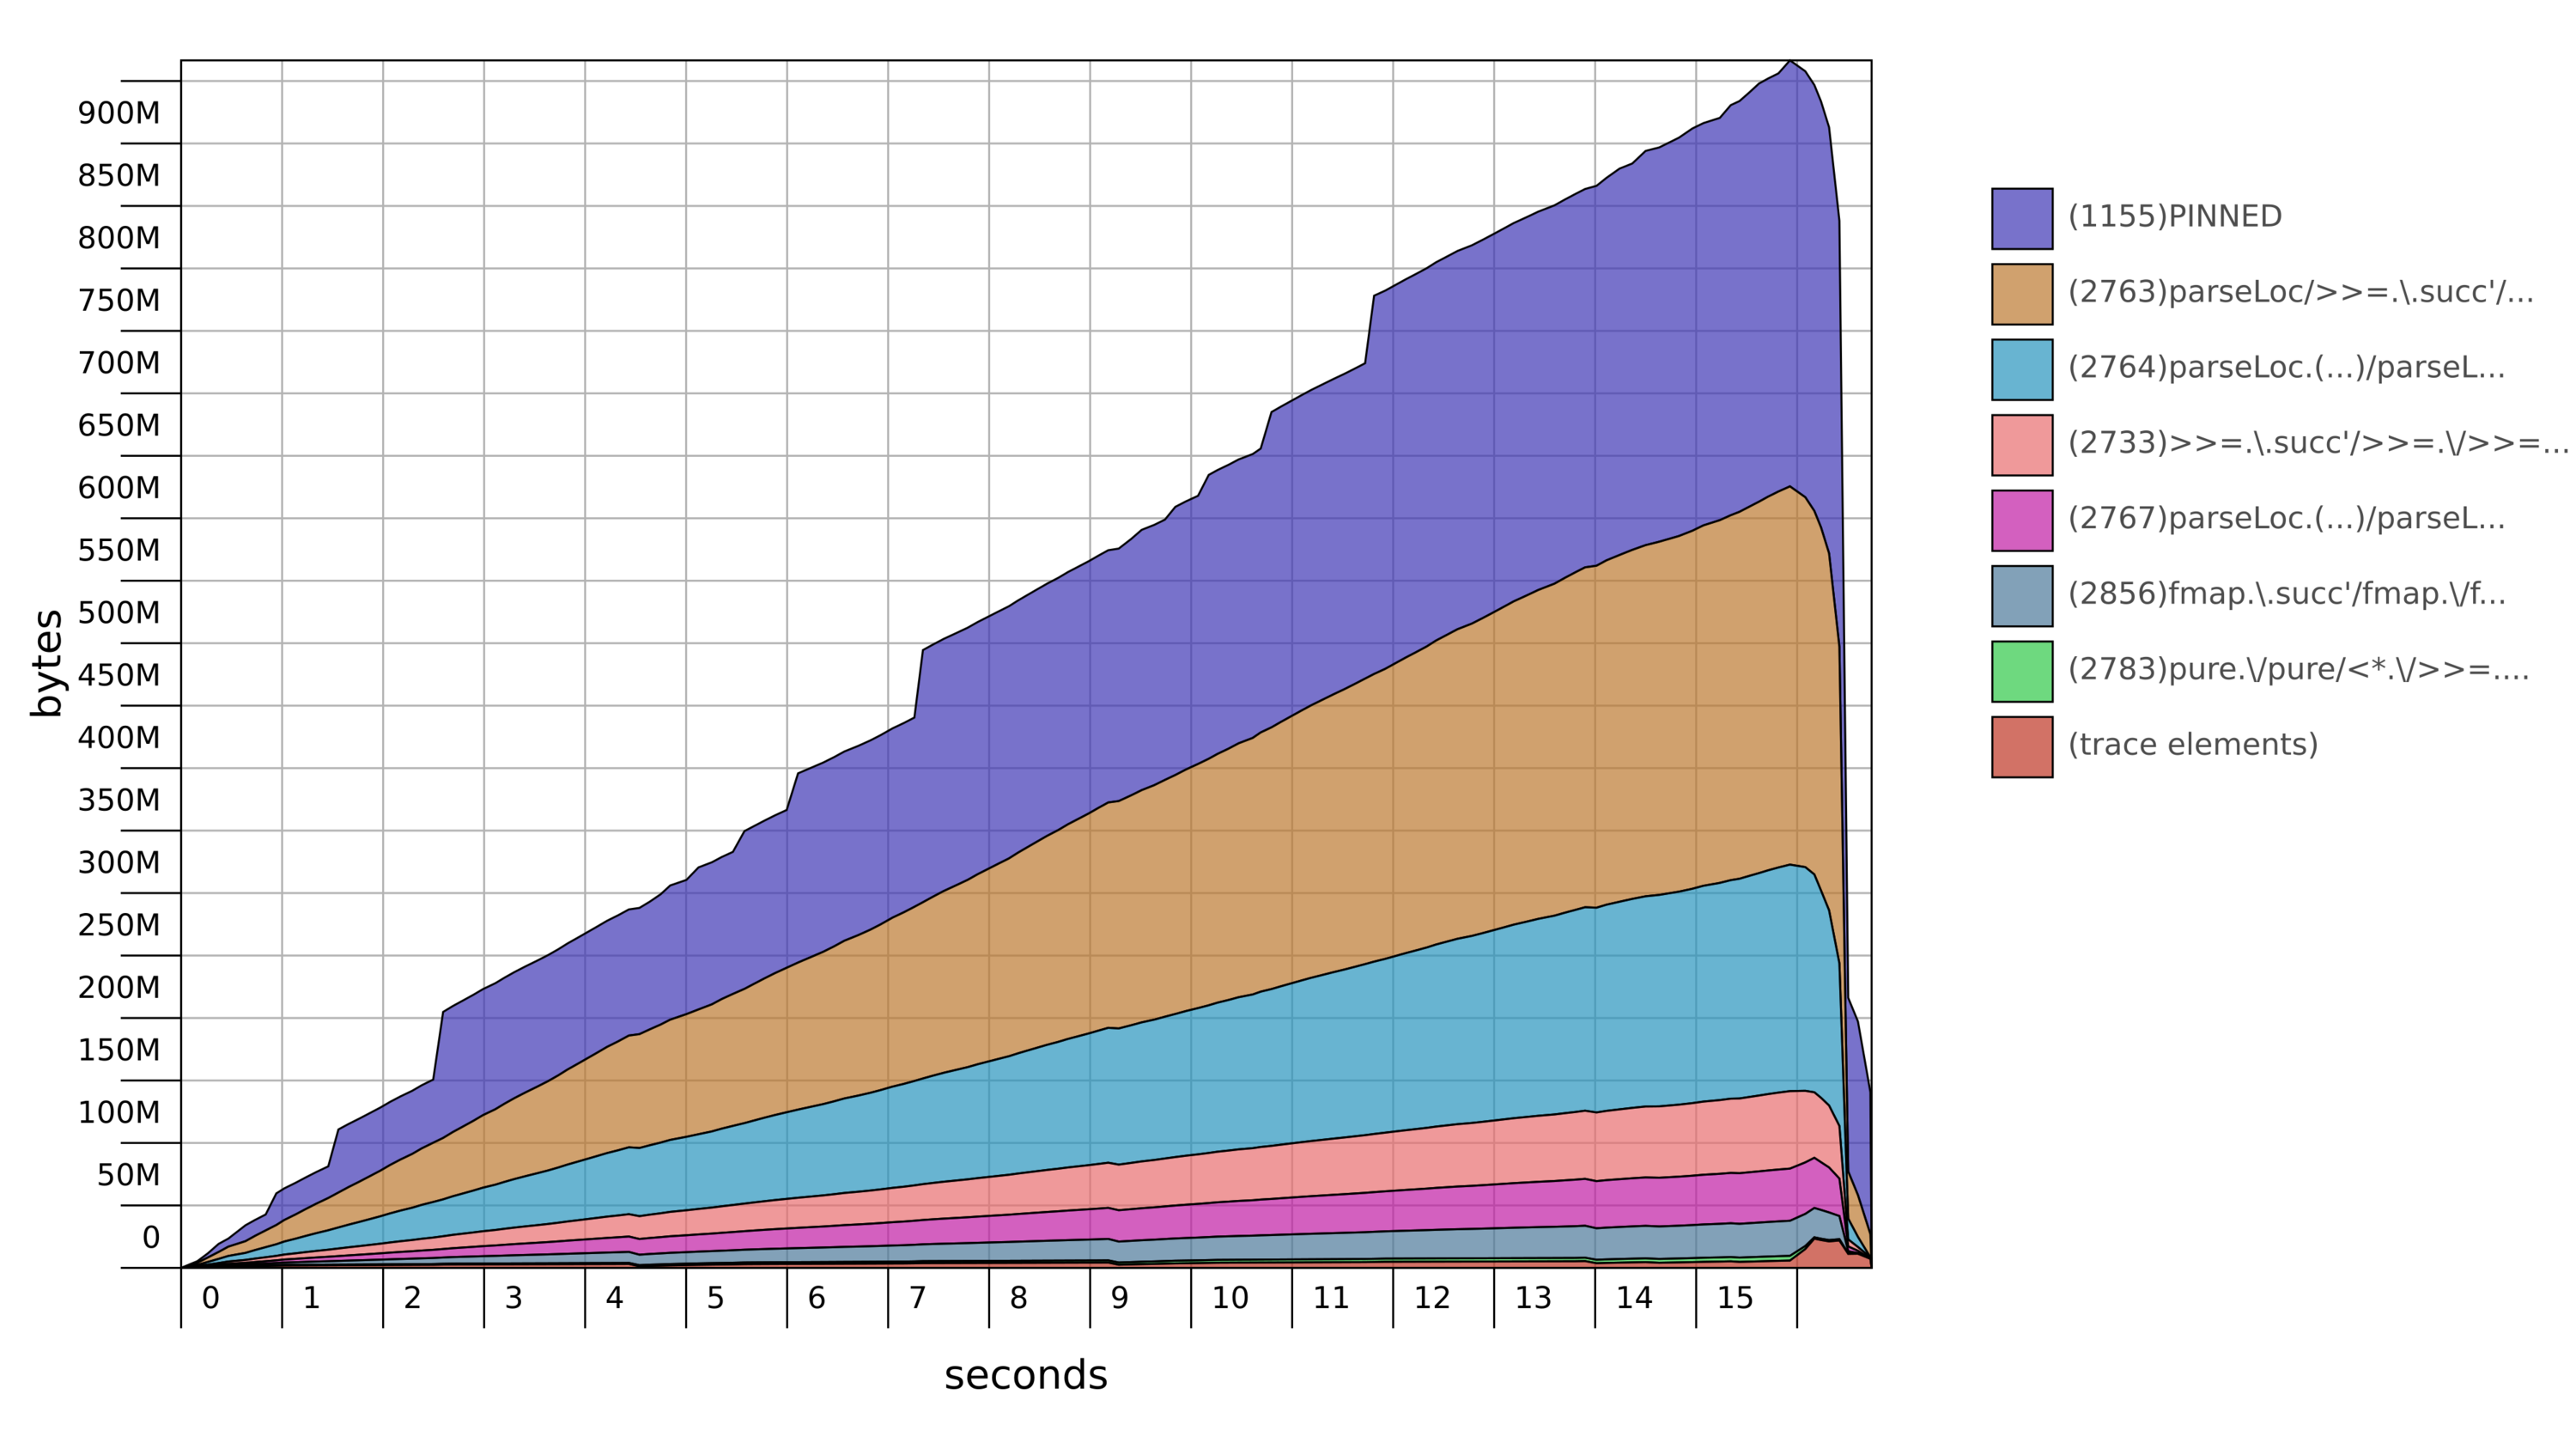
\includegraphics[width=\textwidth]{png/bytestring-lazy}
 \caption{Memory usage of the first implementation using ByteStrings as internal strings representation}
 \label{fig:bytestring-lazy}
\end{figure}

Looking at the diagram, pinned memory seemed to be never freed during the execution. 
Also, traces seemed to reside in memory for too long and occupy too much space. 

The first problem was a reflection of how Haskell keeps \emph{ByteString}s.
They are stored in pinned memory, which is kept on a heap but 
not managed by garbage collector \cite{haskell:shortbytestring-and-text} and cannot be moved around.
As a result, it leads to fragmentation of the heap and cannot be effectively managed.
The fix turned out to be simple. There is a more suitable storage format -- \emph{ShortByteString} 
(also part of the \emph{bytestring} package). It is managed
by GC and stored just like usual heap object, which can be moved around and easily garbage collected.
\footnote{So why even use \emph{ByteString}? Because it is stored in pinned memory, it can be passed to foreign functions.
Also, it is more efficient when the strings are really long and have long livespan}

The second problem was harder to track down. This time the cause was the laziness.
Laziness can improve the perfomance when some objects are never used and the language never needs to fully compute them. 
However, when we know that all objects will eventually be used, it is more efficient
to calculate them as soon as possible. The enforcement of eager evaluation seems to be an obscure
feature, but when we know what is going on, it is fine.
The improvement was visible (figure \ref{fig:shortbytestring-strict}) but it was not the end, 
as peak usage of almost 240MB is still greater than 150MB.

\begin{figure}[hbt!]
 \centering
 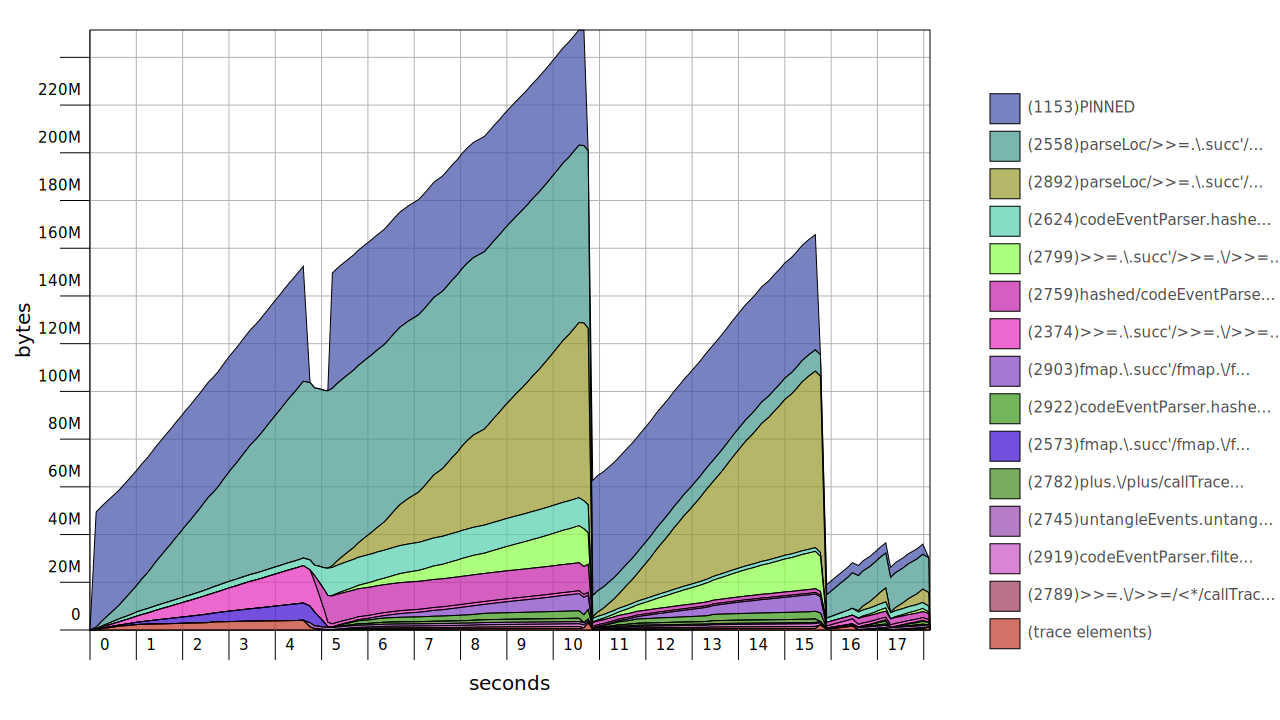
\includegraphics[width=\textwidth]{png/shortbytestring-strict}
 \caption{Memory usage after switching to ShortByteString and forcing eager evaluation}
 \label{fig:shortbytestring-strict}
\end{figure}

It seems suspicious that the entire file has to be kept in memory to be parsed 
(pinned memory on figure \ref{fig:shortbytestring-strict} represents input files read into memory). 
After all, if it was written in C++, probably one line at a time would be read and processed. 
So why this parser consumes so much memory?

This is what \emph{attoparsec} states about incremental input:

\begin{displayquote}
Note: incremental input does not imply that attoparsec will release portions of its internal state for 
garbage collection as it proceeds. Its internal representation is equivalent to a single ByteString: 
if you feed incremental input to a parser, it will require memory proportional to the amount of input you supply. 
(This is necessary to support arbitrary backtracking.)
\end{displayquote}

So, our parser keeps the whole file contents in memory to be able to backtrack. But it is not necessary with
such a simple format. Fortunately, it is possible to improve this behaviour.
Currently, the parser tries to parse the entire file into a list of events. To be sure that it can backtrack,
it keeps the whole input in memory. Instead, we can ask the parser to parse only one event. 
It will do it and return the part of the input that was not parsed yet. We can repeat that in a loop
and parser will never keep more memory that just a few kilobytes. 
Figure \ref{fig:single-event} shows the improvement.

\begin{figure}[hbt!]
 \centering
 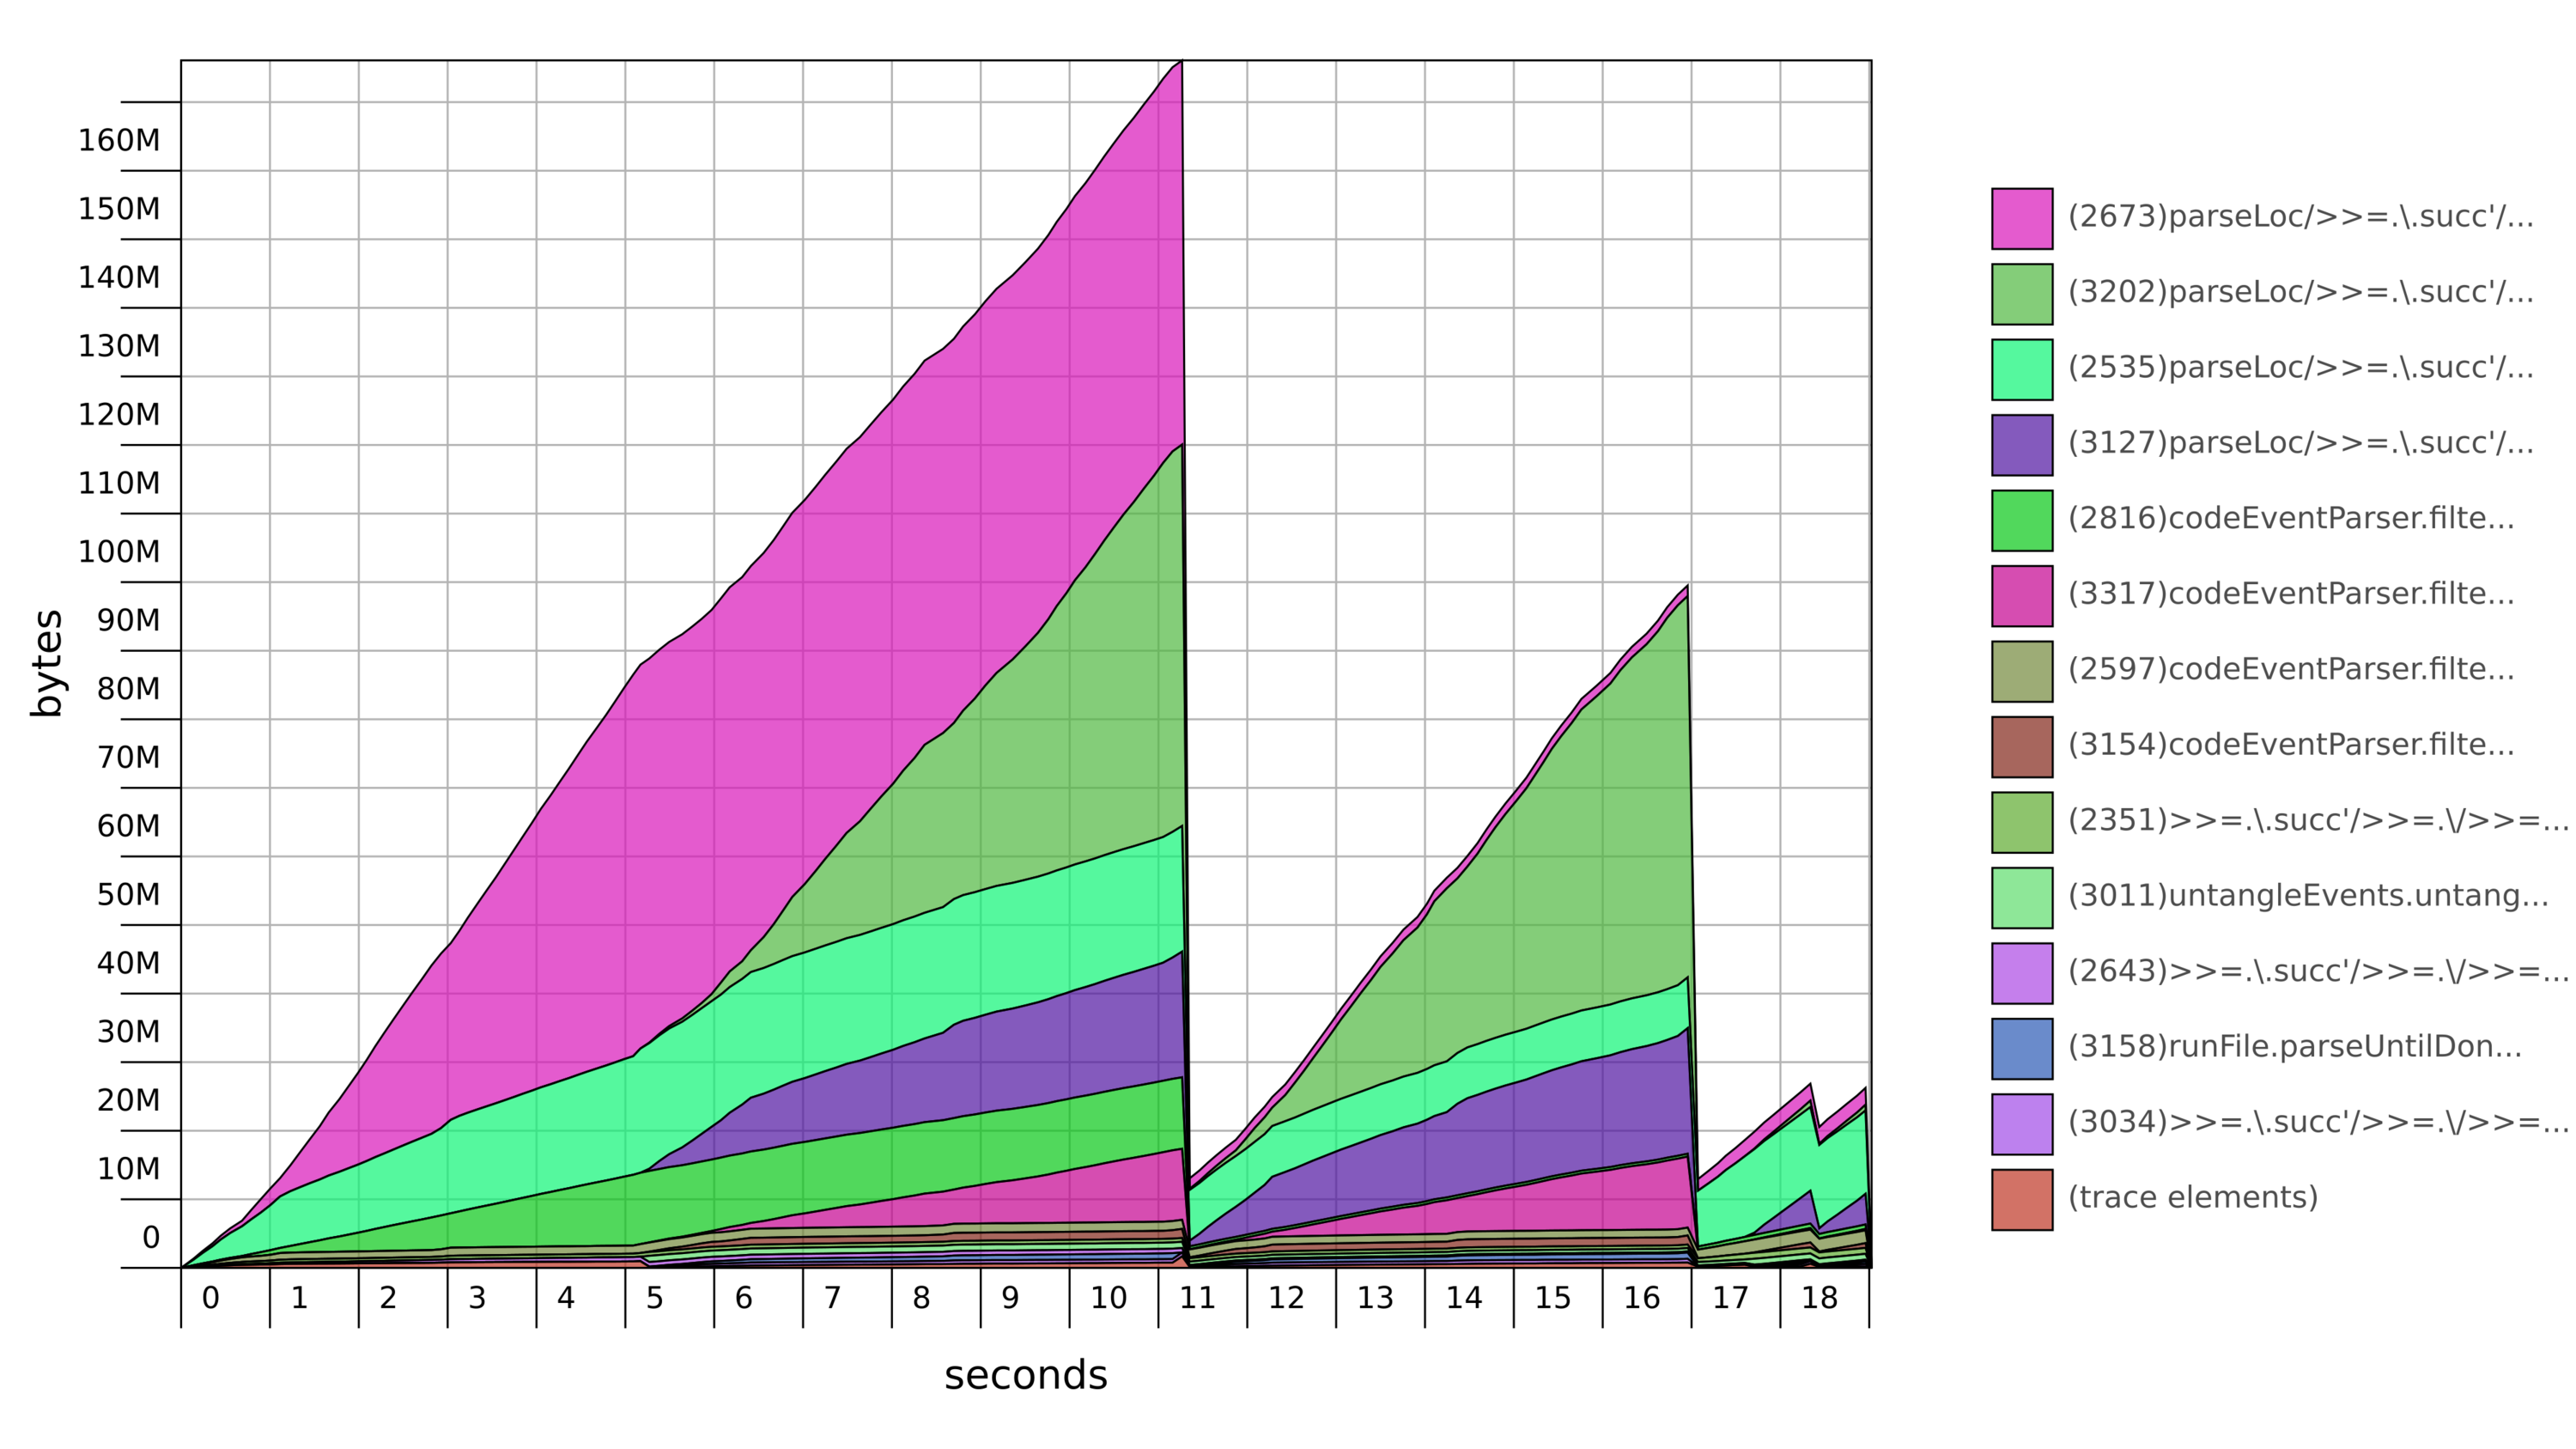
\includegraphics[width=\textwidth]{png/single-event}
 \caption{Memory usage after preventing parser from keeping the entire input file in the memory}
 \label{fig:single-event}
\end{figure}

Last, but not least, the internal representation of the event can be greatly improved.
Locations consist of file names and function names. But both sets are limited!
Usualy there are only a few sources containing just a few hundreds of unique functions. 
We can create a map of all source and function names and just keep appropriate ids in location objects.
Just 4 numbers instead of 2 strings and 2 numbers!

This representation also has another major benefit -- comparisons of such objects are much fasters.

The final memory consumption is presented in figure \ref{fig:strings-map}

\begin{figure}[hbt!]
 \centering
 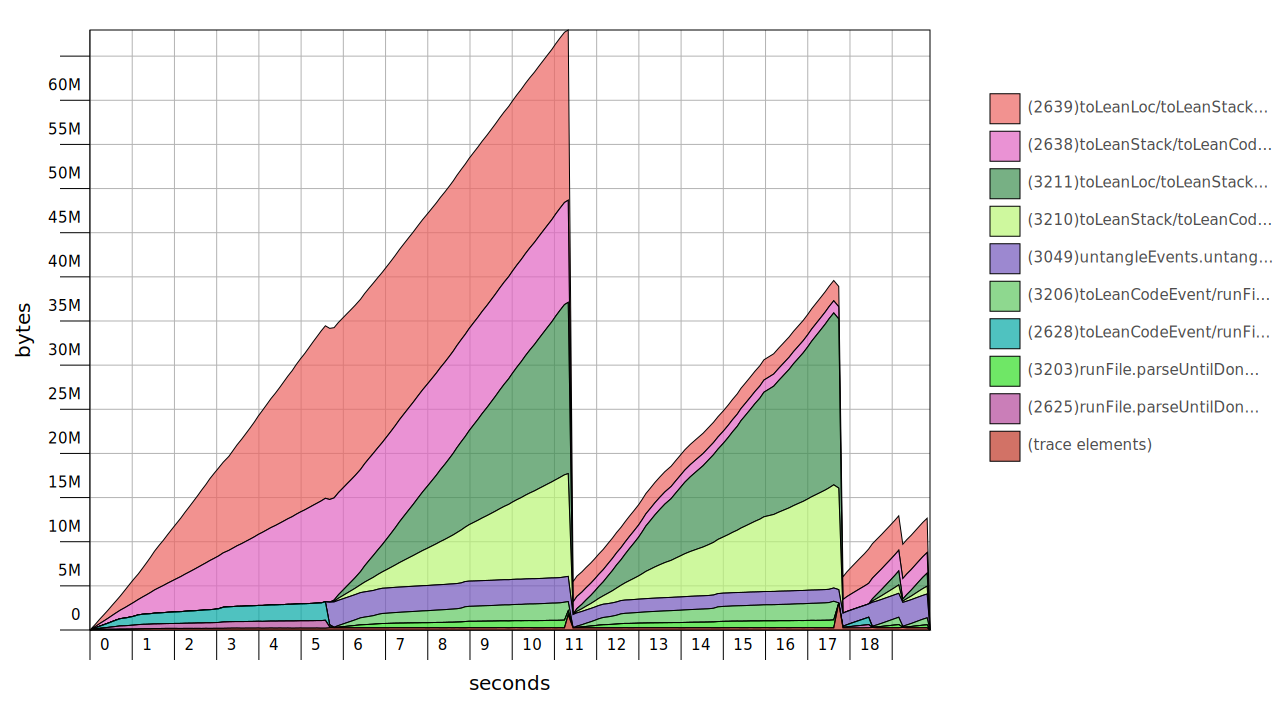
\includegraphics[width=\textwidth]{png/strings-map}
 \caption{Final memory usage}
 \label{fig:strings-map}
\end{figure}


\section{Trace untangling}
Due to the nature of JavaScript execution model (see section \ref{js-exec-model}), execution events
corresponding to different JavaScript events or functions can be intertwined.

For this reason, all events forming a trace have to be untangled into subtraces, each corresponding
to one script or callback. 

Let us recall that all events are logged by our instumented Chromium with their call stacks.
Now, we have three cases:
\begin{itemize}
  \item The event is a function enter with an empty call stack -- it starts a new subtrace
  \item The event is a function exit removing the last item from the stack -- it ends a subtrace
  \item Any other event -- it is a continuation of a subtrace, whose last event has the same call stack
\end{itemize}

Naturally, some care has to be taken to ensure that the right stack is compared. Some events change the
call stack, e.g. function enter and exit, some do not, e.g. "if statement -- then".
Here, the stack \emph{after} the event occured is saved and it is appopriately modified 
(one location can be added, removed or nothing is changed) when comparing
with past events stacks.

Listing \ref{alg-untangling} presents the pseudocode of the algorithm.

\lstinputlisting[language=Pseudocode, caption=Trace untangling, label=alg-untangling, mathescape=true]{algorithms/untangling.alg}

The above code is rather uncomplicated, but it is slow when implemented naively.
The most wasteful part is finding the trace with the right stack in \emph{findMatchingSubtrace}.
To make it faster, two things were done:
\begin{itemize}
  \item Location objects are just 4 numbers instead of 2 strings and 2 numbers. This makes stack comparisons
           one or two orders of magnitude faster
  \item Open traces are kept in a map indexed by stack of the last event. 
  			The lookup becomes logarithmic instead of linear. This optimization is especially important when there are lots
  			of intertwined subtraces. It also must be noted that this optimization alone would not help much if the comparisons 
  			between stacks were slow
\end{itemize} 

\section{Trace alignment}
\label{trace-alignment}

\cite{ieee:alignment-and-slicing}

\section{Trace matching using SMP}

\section{Noise filtering}




\chapter{Evaluation}
\label{evaluation}

In this chapter we give an overview of the implemented system, evaluate it, and present the study
conducted with its help.

\section{The pipeline}

The goal of this work is to automate as many steps of the anti-adblocking analysis as possible.
Ideally, the system should be able to read a list of websites, collect traces, analyze
each of them, and produce meaningful results.

The entire system is brought together by a program written in Python.
It is controlled by an extensive set of flags and logs each step to make troubleshooting easier.
The pipeline comprises the following steps:
\begin{itemize}
  \item A website (or list of websites) to analyze is read as an argument or from a file when a special flag is provided.
  \item If selected, 3 positive and 3 negative traces are collected for each website (before each browser run
           all cookies are deleted). After each run, all unwanted traces are deleted (they may come from extensions 
           or unwanted iframes).
  \item If selected, the analysis is run and results are saved in a selected location.
  \item Optionally, the traces are deleted.
\end{itemize}

The system counts the number of traces with execution differences.
If there is at least one such a pair of traces found, we assume that it is due to the anti-adblocking activities.
The output includes the diff of these traces, as well as all unmatched ones.

\section{Methodology}
\label{methodology}

The methodology is the same as in the original paper \cite{DBLP:conf/ndss/ZhuHQSY18}.
First, we test the effectiveness of the method on sets of negative and positive examples.
Then, we use the system to conduct a small scale study.

One important difference compared to the original approach is that, unless the page has a visible anti-adblocking
reaction on the main page, we always test the websites on their subpages. The reason is that
some news pages show the anti-adblocking warnings only in the articles.

The authors of the original work composed the negative examples set from 100 websites that do not display ads.
The reasoning behind this is that they are guaranteed not to contain any anti-adblocking scripts.
However, such a choice of examples as a benchmark seems flawed.
One of the key challenges in this method is the noise filtering. If there are no ads, 
then there are practically no sources of execution differences between runs with and without an adblocker.
A better choice of websites to evaluate an anti-adblock detection system on would be a mix of websites without ads and sites that
display ads, but are known to contain no anti-adblockers.
Unfortunately, finding such websites is not easy as it entails a detailed analysis of the entire code
served by each site. Certainly, it is not a task for one person to be done in a reasonable timespan.
For this reason, we also only consider pages that do not serve ads, exactly 50 of them, as the negative examples.

Zhu et al. \cite{DBLP:conf/ndss/ZhuHQSY18} have an extensive list of websites with anti-adblockers collected during their
previous studies (almost 700 positions). Unfortunately, they do not share this list. 
For this reason, a similar list of positive examples had to be created from scratch.
It is a mix of websites encountered during daily browsing and sites appearing in the
Polish anti-adblock filter list \cite{github:anti-adblock-list}.
To avoid a time-consuming code analysis at the stage of composing the list, 
all selected websites contain visible anti-adblocking warnings.
Another important note is that the list contains at most a handful of websites 
from Alexa 500 list \cite{alexa-list} to keep the list
usable for the small scale study.

The ad-blocking extensions have different policies when it comes to their official, default filters.
AdBlock Plus behaves politely and respects publishers' right to ask users to show some support
and disable the extension, whatever form such a request takes \cite{adblock:policy}.
On the other hand, uBlock Origin employs a different rule. If the warning is not dismissable or is annoying,
it is blocked \cite{vice:ublock-policy}.

Since usage of AdBlock Plus may expose a wider variety of adblock walls and warnings, 
it was chosen for the experiments.

\section{Negative examples}

The list of websites without ads, on which the system was tested is presented in Table \ref{table:negative}.
The number of execution differences found is listed in the last column.

\csvreader[webisteList,
  longtable= r | p{13cm} | r ,
  table head=\caption{Results of a system evaluation on the negative examples -- pages without ads}
  \label{table:negative}\\
  \hline & URL & \thead{Diff. \\ count}\\\hline
]{tsv/negative.tsv}{}%
{\thecsvrow & \url{\adr} & \cnt}%

Ideally, there should be no execution differences on any website listed here. Nonetheless, 
a few differences were identified (positions 44-50).
We comment on them below.

\subsubsection{\url{kinoelektronik.pl}}
The origin of the difference is unclear. There does not seem to be any element
blocked by AdBlock. Also, there are no blocked network requests. 
But, for some reason, there are differences in jQuery traversals.

\subsubsection{\url{ethz.ch}}
The cause of the difference is the tracking code.

\subsubsection{\url{szkolaimpro.pl}}
The difference is due to the progress bar.

\subsubsection{\url{www.paperswithcode.com}}
The execution divergence stems from Sentry -- an error reporting solution.

\subsubsection{\url{www.whitehouse.gov}}
The origin of the difference is unclear.

\subsubsection{\url{www.worldanimalprotection.org}}
A similar case to \url{kinoelektronik.pl}. The difference is reflected in jQuery traversals
but it is unknown why the DOM trees are different.

\subsubsection{\url{zoo.waw.pl}}
The same case as in \url{kinoelektronik.pl} and \url{www.worldanimalprotection.org}.


\section{Positive examples}

For the positive case evaluation, we run the system on 50 websites that contain visible anti-adblocking warnings.
Afterwards, we manually inspected each page and verified if the differences found by the system were relevant.

The results are presented in Table \ref{table:positive}.
Each row consists of a URL, a number of traces with execution divergences, a relevance of the differences,
and an anti-adblocker type.

In most cases the system is able to find execution differences, which is a very good sign.
In the following sections we analyze when the system fails and discuss
how the detected solutions work.

The analysis of 50 websites incorporating adblock walls allows us to create a simple
classification of anti-adblocking mechanisms:
\begin{itemize}
  \item Bait-based
    \begin{itemize}
     \item A file as a bait
       \begin{itemize}
         \item A variable value is changed
         \item An element injected into the DOM
         \item An error handler on a network request
       \end{itemize}
     \item A DOM element as a bait
    \end{itemize}
  \item Real ads checkup
    \begin{itemize}
      \item A visibility inspection
      \item A load verification
    \end{itemize}
\end{itemize}

We can also enumerate all encountered anti-adblocking solutions:
\begin{itemize}
  \item Custom scripts
  \item Off-the-shelf modules:
    \begin{itemize}
      \item BlockAdBlock \cite{github:blockadblock}
      \item Adblock Detect \cite{adblock-detect}
      \item Kill AdBlock \cite{kill-adblock}
      \item Admiral's Recover \cite{admiral:recover}
      \item \emph{an\_message\_display}
      \item \emph{Adb\_Detector}
    \end{itemize}
\end{itemize}

The most popular solutions are custom scripts and open-source BlockAdBlock (already mentioned in Section \ref{anti-adblockers}).
Other open-source scripts include Adblock Detect and KillAdBlock. One website also used a paid solution -- the Admiral platform.
The origin of the last two solutions is unclear, but the code was clearly the same (the names listed are 
distinctive functions' names, not the real names of these modules).

Some custom scripts can be really widespread -- some publishers own a number of domains and it makes 
sense to create one robust solution and use it in every website. One example is the Wirtualna Polska group (positions 25 and 27), 
which uses their own custom anti-adblocking module.

In most cases a significant part of the differences found originated from third-party ads
or tracking code (Google Analytics, AdWords, Gemius trackers, Twitter buttons, Facebook buttons, etc.),
but it was not inspected further.

\csvreader[webisteList,
  longtable= r | p{8cm} | r | c | p{4cm} ,
  table head=\caption{Results of a system evaluation on the positive examples -- pages with adblock walls}
  \label{table:positive}\\
  \hline & URL & \thead{Diff. \\ count} & \thead{Diff \\ rel.?} & Type\\\hline
]{tsv/positive.tsv}{}%
{\thecsvrow & \url{\adr} & \cnt & \res & \type}%


\subsection{Websites with unsatisfactory results}

\subsubsection{\url{jakimasklad.pl}}
A brief analysis of the code shows that the site incorporates BlockAdBlock \cite{github:blockadblock}. 
It turns out that, in this case the module's obfuscation is effective enough to circumvent our system.
It is interesting that a number of different websites use the same solution and the system
is able to pinpoint the differences in these cases.

\subsubsection{\url{www.srebrnestawy.pl}}
In this case the code that activates the warning seems very simple and there is no reason why
it should not be detected by the system. Listing \ref{js:srebrnestawy} shows the code.

\lstinputlisting[language=JavaScript, caption=An anti-adblocking script of \url{www.srebrnestawy.pl}, 
                       label=js:srebrnestawy]{js/srebrnestawy.js}

The reason why it is not detected is that the bait is based on the file \emph{advert.js}, which is not loaded 
even when AdBlock is disabled, due to an HTTP 404 error. Consequently, the warning is displayed even 
when AdBlock is disabled and the system is right -- there are no execution differences.

\subsubsection{\url{www.cyberciti.biz}}
In this case the difference found corresponds to a PageAd reaction,
but the check that activates the adblock warnings is not found.

An anti-adblocker used on this page is simple, works in the same way as the one found on site \url{www.audiklub.pl}.
This site, however, uses Cloudflare's Rocket Loader \cite{cloud-flare:rocket-loader}.

Rocket Loader is a powerful mechanism, developed by Cloudflare, that is able to cache JavaScript code and defer its execution 
until the entire web page is rendered. The way it works is the following: 
\begin{itemize}
  \item  Before serving the page, the server inspects the website and changes all JS scripts 
            to some type not identified by the browser as JavaScript code.
            The type also has to be unique so that these scripts are easy to find later.
  \item The server also encloses a special JavaScript module that activates when the entire web page is loaded.
  \item JavaScript module finds all scripts with changed type and executes them.
\end{itemize}

Since the module that executes the scripts is JavaScript code, the system should still be able
to detect the anti-adblocking code. Unfortunately, it did not manage to do so 
and the most probable reason seems to be a bit aggressive noise filtering. 
If some function performs a DOM traversal and
the content changes a little each time the page is loaded, it is probable that it is filtered out.
We suspect that it is the case here. That is, Rocker Loader has to find all scripts (a DOM traversal) and execute them
as a part of one long function.

\subsubsection{\url{torrentcity.pl}}
This is an example of a rather sophisticated custom anti-adblocking script.
Listing \ref{js:torrentcity} shows the code that performs the check.

\lstinputlisting[language=JavaScript, caption=An anti-adblocking script of \url{torrentcity.pl}, 
                       label=js:torrentcity]{js/torrentcity.js}
                       
The script first sets up a bait by injecting a new script element into the DOM. It is set up to download
a file named \emph{ads.js}, which should be blocked by any adblocker.

Next, the error handler is set up to activate the reaction. If the load succeeds, it still
makes sure that the ads are actually displayed.

Functions called as event handlers or via \emph{setTimeout} are a weak spot of 
the Differential Execution Analysis method, not just this exact implementation 
and there is no known way to automatically utilize such unpaired events.

\subsubsection{\url{player.pl}}
An example of a really robust solution, probably used on every site belonging to the TVN media company.
Listing \ref{js:tvn} shows the checks. The website utilizes more than one check
to increase the detection effectiveness.
The checks itself are similar to what we have already seen. The first one creates an element as a bait 
and checks if it is visible. The second one uses a different bait, a file, and reacts within callbacks.
The system fails here because the script uses the techniques 
that are the weak spot of the presented method.

\lstinputlisting[language=JavaScript, caption=An anti-adblocking script of \url{player.pl}, 
                       label=js:tvn]{js/tvn.js}

\subsubsection{Other websites}
In cases of other websites where the relevant execution divergences were not found 
the reasons were the same -- either the check was intertwined between other activities
in a way that filtering would discard it or the check was fired via callbacks.


\subsection{Detected anti-adblockers}

This section presents some interesting mechanisms 
that have not been covered yet but have been detected.
Simple examples were preferred to avoid showing cluttered code.

\subsubsection{\url{www.audiklub.pl}}
\label{audiklub}
This is the simplest anti-adblocking script one can think of. The website includes just one advertisement, 
but when an adblocker is detected, the entire content is blocked (Listing \ref{js:audiklub}).

\lstinputlisting[language=JavaScript, caption=An anti-adblocking script of \url{www.audiklub.pl}, 
                       label=js:audiklub]{js/audiklub.org.js}

First, the trap is set up. It is a file named \emph{ads.js}.
Its content is just one line which sets the \emph{canRunAds} variable to true.

The main check is performed in the \emph{window.onload} callback. The script simply checks
if the \emph{canRunAds} variable has been set. If not, it replaces the content div with an anti-adblocking warning.

\subsubsection{\url{kursbootstrap.pl}}
The script on this website serves as an example of an anti-adblocker that uses a file as a bait
but the check is performed by injecting an element into the DOM instead of setting a global variable
(Listing \ref{js:kursbootstrap}).

\lstinputlisting[language=JavaScript, caption=An anti-adblocking script of \url{kursbootstrap.pl}, 
                       label=js:kursbootstrap]{js/kursbootstrap.js}
                       
\subsubsection{\url{who-called.eu}}
The code from this website demonstrates how an anti-adblocking script can detect if real
ads are displayed, without using a bait (Listing \ref{js:whocalled}).
The detecting function is run 5 seconds after the page finishes loading. It then checks if the content 
of the element displaying ads is empty (contains 0 non-whitespace characters).

\lstinputlisting[language=JavaScript, caption=An anti-adblocking script of \url{who-called.eu}, 
                       label=js:whocalled]{js/whocalled.js}
                       
\subsubsection{\url{kimcartoon.to}}
This website employs a check based on making sure that advertising scripts
are loaded (Listing \ref{js:kimcartoon}). It seems, though, that the code contains a bug.
Perhaps it would be desirable to invert the condition and change the variable
only when one of the scripts fails to load (currently it is enough that one of them is loaded correctly)

\lstinputlisting[language=JavaScript, caption=An anti-adblocking script of \url{kimcartoon.to}, 
                       label=js:kimcartoon]{js/kimcartoon.js}
                       
\subsubsection{\url{e-dokument.org} and others using BlockAdBlock with \emph{eval} obfuscation}
BlockAdBlock is one of the most popular off-the-shelf anti-adblocking solutions.
The obfuscated code is quite unreadable to a human (Listing \ref{js:edokument}).
Fortunately, the string to be evaluated contains "BlockAdBlock" as a substring and we can be sure that it was
the solution used. Since BlockAdBlock is an open-source module, an interested reader can check 
out its code in the plain, unobfuscated form on github \cite{github:blockadblock}.

\lstinputlisting[language=JavaScript, caption=An anti-adblocking script of \url{e-dokument.org}, 
                       label=js:edokument]{js/edokument.js}

\subsubsection{\url{polscygracze.pl}}
Another website that uses BlockAdBlock, but adds a fallback in case the module is blocked
by an adblocker (Listing \ref{js:polscygracze}). It is worth mentioning that the idea of 
making the id of the adblock warning element random is good but the identifier should be dynamic,
i.e., generated randomly each time the page is loaded.
If it is static, it can still be added to adblockers' filter lists.
                       
\lstinputlisting[language=JavaScript, caption=An anti-adblocking script of \url{polscygracze.pl}, 
                       label=js:polscygracze]{js/polscygracze.js}

\subsubsection{Other off-the-shelf solutions}
Other solutions utilize mechanisms similar to the already described ones.
They can be more polished and use more than one check
but they do not introduce any new ideas. For this reason they are not described further here.
An interested reader can check their documentation.


\section{Small scale study}

The experiment has been conducted on almost 300 top websites from Alexa 500 list (the version for Poland) \cite{alexa-list}.
The list of the visited websites and the results is attached in Appendix A. Some websites were skipped because they
either contain adult content or their main domain does not contain any web page 
-- this is the case, e.g., for content delivery networks.
These websites, instead of results, contain dashes (\texttt{-{}-}) in the last two columns.

Some results are marked with "TO" (timeout) instead of a number of differences found. This is because
there is a limited time for each trace collection (30 seconds). After that the browser is closed.
In some cases the browser times out instead of closing. The system then waits another 90 seconds and closes
the browser forcefully.
Usually this is a sign of a website producing an enormously large execution trace
(some can reach almost 50GB in 2 minutes). Such pages are also skipped.

Although the number of ads, social media links and similar elements was not counted, it seems that the more 
elements of this kind a website incorporates, the more likely it is that there will be an anti-adblocking reaction of some kind.
It is especially true in case of third-party ads which more often than not report an adblocker presence.

Out of 281 visited websites, 33 contained visible anti-adblocking warnings. 
The system detected anti-adblocking reactions in 163 web pages, 103 were found to be free of anti-adblockers.
The rest (15 pages) timed out.
Looking at the results, it seems that the anti-adblocking scripts are widespread. 
Silent anti-adblocking reactions are over 5 times more frequent than adblock walls
(163 reactions detected vs 33 adblock walls detected). Over 50\% of the visited websites exhibit some sort of
anti-adblocking reactions. It is not that surprising if we consider that most websites contain advertisements
and the biggest ad providers report adblockers usage.


\section{Conclusion}

The performed tests show that the system is capable of detecting the anti-adblocking scripts in many scenarios.
The exact numbers are not presented purposefully -- the tests should be conducted on larger set of websites
and the methodology should be different when it comes to the negative examples.

The presented solution certainly has some weak spots. The first one is the event coverage. 
It is easy to hide anti-adblockers by utilizing callbacks. The second one is the data 
filtering mechanism which in some cases may filter out too much data,
and in others it lets through too many traces, which limits its usefulness (the analysis becomes much harder,
the optimum would be to always have less that 10 trace diffs for manual verification).

Here are some ideas that could alleviate both problems:
\begin{itemize}
  \item Make an extension that would put a thin wrapper around some critical built-in functions. Such wrapper would only
           call the original built-in function but the entry and the exit would be logged by the system.
           It might be useful for functions such as \emph{getElementById} or direct DOM manipulations.
  \item Manually analyze and tag the results of more traces (at least hundreds of them) 
           and try some machine learning method to filter the resulting diffs. 
           A first try could be to use the random decision forests.
\end{itemize}

The system is also a bit too slow. The trace collection should have less overhead on the browser. 
For a large scale study spending 10 minutes on each website to collect traces is too long.
One idea is to have Chromium assemble a strings map instead of constructing it the during analysis. 
This, in conjunction with a use of some binary format, would
result in much more compact files and less time wasted on writing to files.

Last but not least, the conducted experiments give lots of insights on how to build an effective anti-adblocker:
\begin{itemize}
  \item Use more than one detection method, preferably utilizing callbacks.
  \item Obfuscate the code by using minification combined with the \emph{eval} function to make manual analysis extremely hard.
  \item Randomize ids of injected adblock warnings to make it harder for the adblockers to filter them out.
\end{itemize}



\lstlistoflistings
\addcontentsline{toc}{chapter}{Listings}

\listoffigures
\addcontentsline{toc}{chapter}{List of Figures}

\listoftables
\addcontentsline{toc}{chapter}{List of Tables}

\cleardoublepage
\phantomsection
\addcontentsline{toc}{chapter}{Bibliography}
\bibliography{sources}{}
\bibliographystyle{plain}

\chapter*{Appendix A}
\addcontentsline{toc}{chapter}{Appendix A}

\csvreader[webisteList,
  longtable= r | p{12cm} | c | r ,
  table head=\hline & URL & \thead{Vis. \\ warn.} & \thead{Diff. \\ count}\\\hline
]{tsv/alexa.tsv}{}%
{\thecsvrow & \url{\adr} & \wall & \cnt}%

\end{document}


%%% Local Variables:
%%% mode: latex
%%% TeX-master: t
%%% coding: latin-2
%%% End:
